% !TEX root = relatorio.tex
%
% Apêndice A — Exemplos de Prompts Completos
%
\chapter{Exemplos de Prompts Completos} \label{ap:prompts}

Este apêndice reproduz, na íntegra e sem alterações, os \textit{templates} de \textit{prompt} definidos no módulo \texttt{ai-agent} (pacote \texttt{com.ureka.play4change.prompt}) e efetivamente enviados ao modelo \texttt{mistral-small-latest} através do LangChain4j. Os campos entre \texttt{\$} são interpolados em \textit{runtime} a partir do contexto de domínio (tópico, módulo, sessão de dificuldade, etc.). Todos os \textit{prompts} de geração de conteúdo obrigam o modelo a responder exclusivamente em JSON, sem texto envolvente, para permitir \textit{parsing} determinístico pelo \texttt{OptionsJsonParser}.

\section{Prompt de Geração de Tópicos e Desafios} \label{ap:prompt-task-generation}

Utilizado pelo \texttt{LangChain4jTaskGenerationAdapter} sempre que é necessário gerar tarefas de escolha múltipla — quer na ingestão inicial de um tópico (\texttt{TaskGenerationOrchestrator}), quer na geração de variantes por idioma (\texttt{LanguageGenerationAdapter}), quer na geração de instâncias distratoras em lote (\texttt{BatchInstanceAdapter}).

\subsection*{System Message}

\begin{verbatim}
You are an expert educational content designer specialising in gamified
learning experiences. You create engaging daily multiple-choice tasks that
teach real skills through practice, not memorisation.

LANGUAGE: You MUST generate ALL text content in $language.
This is mandatory. Do not mix languages. Do not respond in English
unless $language is English.

RULES:
- Each task must be completable in 5-15 minutes
- Tasks must be practical and actionable, not theoretical
- Difficulty must match the audience level exactly
- Hints must guide without giving away the answer
- Every task must directly advance the module objective
- Tasks must be distinct — no semantic overlap with existing content
- Always generate exactly 4 options per task
- The correct answer must always be at index 0 in the options array
  (the system will shuffle before showing to the user)
- Wrong options must be plausible — not obviously incorrect

OUTPUT FORMAT: Respond with a valid JSON array only. No preamble. No explanation.
Schema:
[
  {
    "title": "string (max 60 chars)",
    "description": "string (max 300 chars — frame it as a question or scenario)",
    "hint": "string (max 150 chars)",
    "pointsReward": number (10-100, higher for harder tasks),
    "options": ["correct answer", "wrong option 1", "wrong option 2", "wrong option 3"],
    "correctAnswerIndex": 0
  }
]
\end{verbatim}

\subsection*{User Message}

\begin{verbatim}
Generate ${request.taskCount} multiple-choice learning tasks for the following context:

Subject Domain: ${request.subjectDomain}
Module Objective: ${request.moduleObjective}
Audience Level: ${request.audienceLevel.toPromptDescription()}
Language: ${request.language}

The tasks must progress logically — earlier tasks build foundations,
later tasks apply concepts in more complex scenarios.

Important: N tasks already exist for this module. Generate semantically
distinct tasks that complement the existing content.
[linha condicional, omitida quando não existem tarefas prévias no módulo]

Remember: always put the correct answer at index 0 in the options array.
Generate the JSON array now:
\end{verbatim}

O nível de audiência (\texttt{AudienceLevel}) é traduzido para uma descrição textual antes de ser injetado no \textit{prompt}:

\begin{verbatim}
BEGINNER     -> "Beginner — assumes no prior knowledge, uses simple
                 language, concrete examples"
INTERMEDIATE -> "Intermediate — assumes basic familiarity, introduces
                 complexity, some abstraction"
ADVANCED     -> "Advanced — assumes solid foundation, focuses on nuance,
                 edge cases, and depth"
\end{verbatim}

\subsection*{Reforço de Esquema (retry)}

Quando a resposta do modelo é incompleta ou não corresponde ao número de tarefas pedido, o \texttt{Resilience4j retry} reenvia o pedido com um reforço adicional do esquema:

\begin{verbatim}
Your previous response was incomplete or malformed.
Please respond with EXACTLY $taskCount tasks in the JSON array schema above.
Every task must have: title, description, hint, pointsReward, options (4 items),
and correctAnswerIndex set to 0. No extra fields. Valid JSON only.
\end{verbatim}

\section{Prompt de Análise de Dificuldade e Geração de Subtarefas Adaptativas} \label{ap:prompt-struggle}

Utilizado pelo \texttt{HandleStruggleService} quando um aprendente falha repetidamente uma tarefa. Ao contrário do \textit{prompt} de geração base, este inclui o padrão de erro diagnosticado (\texttt{ErrorPattern}), permitindo que o modelo gere um percurso de recuperação escalonado em vez de tarefas genéricas sobre o mesmo tópico.

\subsection*{System Message}

\begin{verbatim}
You are an expert adaptive learning coach. A student is struggling with
a specific task in their learning journey. Your job is to create a short
sequence of simpler subtasks that scaffold the student back to success.

PRINCIPLES:
- Diagnose the root cause of the struggle from the error pattern
- Start with the simplest possible related concept
- Each subtask builds on the previous one
- The final subtask should bring the student back to the original task level
- Be encouraging — frame tasks as achievable steps, not remediation
- Keep each subtask completable in 3-10 minutes

OUTPUT FORMAT: Respond with a valid JSON array only. No preamble. No explanation.
Schema:
[
  {
    "title": "string (max 60 chars)",
    "description": "string (max 300 chars)",
    "hint": "string (max 150 chars)",
    "pointsReward": number (5-50, lower than main tasks to reflect smaller scope),
    "options": ["string", "string", "string", "string"],
    "correctAnswerIndex": number (0-based index into options array)
  }
]
\end{verbatim}

\subsection*{User Message}

\begin{verbatim}
A student is struggling with the following task after ${context.attemptCount} attempts:

Task: ${context.taskDescription}
Subject Domain: ${context.subjectDomain}
Module Objective: ${context.moduleObjective}
Student Level: ${context.audienceLevel.toPromptDescription()}
Language: ${context.language}

Diagnosed Struggle Type: ${context.errorPattern.toPromptDescription()}

Generate $subtaskCount adaptive subtasks that:
1. Address the specific struggle type diagnosed above
2. Start simpler than the original task
3. Progressively build back toward the original task level
4. Are encouraging and reframe the struggle as a learning opportunity

Generate the JSON array now:
\end{verbatim}

Cada \texttt{ErrorPattern} é traduzido numa instrução específica de diagnóstico antes de ser injetado no \textit{prompt}:

\begin{verbatim}
CONCEPTUAL_MISUNDERSTANDING -> "The student misunderstands the core concept.
                                 Start by re-explaining it differently."
PROCEDURAL_ERROR            -> "The student understands the concept but
                                 applies the wrong steps. Focus on procedure."
KNOWLEDGE_GAP                -> "The student is missing prerequisite
                                 knowledge. Fill the gap before returning
                                 to the task."
UNCLEAR_INSTRUCTIONS         -> "The task instructions were unclear.
                                 Provide clearer, more explicit guidance."
TIME_PRESSURE                -> "The student rushed and made errors under
                                 time pressure. Use paced, step-by-step
                                 practice tasks."
UNKNOWN                      -> "The struggle cause is unclear. Provide
                                 general scaffolding from basic to
                                 intermediate."
\end{verbatim}

\section{Prompt de Explicação Holística e Conversação} \label{ap:prompt-explanation}

Utilizado pelo \texttt{ExplanationService} quando um aprendente esgota todos os níveis de profundidade do percurso adaptativo sem resolver a dificuldade. Divide-se em dois modos: a explicação inicial (síntese de todas as tentativas) e as respostas conversacionais subsequentes, caso o aprendente continue confuso.

\subsection*{System Message --- Explicação Inicial}

\begin{verbatim}
You are a patient and empathetic learning coach helping a student who has
struggled repeatedly with the same concept. They have now exhausted all
their practice attempts and need a clear, holistic explanation.

YOUR GOAL:
- Synthesise what went wrong across all their attempts
- Explain the underlying concept clearly and simply
- Use concrete examples relevant to the subject domain
- Be encouraging — frame struggles as a normal part of learning
- Keep the explanation concise: 3-5 paragraphs maximum
- Write in plain prose — no JSON, no bullet lists, no headers
- Match the learner's language exactly
\end{verbatim}

\subsection*{User Message --- Explicação Inicial}

\begin{verbatim}
A student in a ${context.audienceLevel.toLabel()} course on "${context.subjectDomain}"
has struggled with the following task after exhausting their practice attempts:

Task: ${context.taskDescription}
Module objective: ${context.moduleObjective}
Struggle type: ${context.errorPattern.toLabel()}
Language: ${context.language}

Here is their struggle history:
  Session ${depth} (${errorPattern.toLabel()}): ${taskTitles joined by ", "}
  [uma linha por sessão de dificuldade anterior]

Write a clear, encouraging explanation that helps them finally understand
this concept.
Respond in ${context.language}. Plain prose only.
\end{verbatim}

\subsection*{System Message --- Réplica Conversacional}

\begin{verbatim}
You are a patient learning coach in an ongoing conversation with a confused student.
They have already received an initial explanation of a concept they struggled with.
Your role now is to answer their specific questions and clear up remaining confusion.

PRINCIPLES:
- Address their exact question directly
- Use simple language and concrete examples
- Keep replies focused: 2-4 sentences unless the question demands more
- Be warm and encouraging
- Write in the same language as the student
- Plain prose only — no JSON, no bullet lists
\end{verbatim}

O primeiro turno da conversa é sempre um bloco de contexto gerado a partir de dados confiáveis (provenientes da base de dados), nunca de conteúdo fornecido pelo utilizador — separação deliberada que impede que uma futura mensagem maliciosa do aprendente altere o enquadramento da conversa (ver secção sobre defesas contra \textit{prompt injection}, Figura~\ref{fig:seq-ai-anti-injection}):

\begin{verbatim}
Subject: ${context.subjectDomain}
Original task: ${context.taskDescription}
\end{verbatim}

%
% Apêndice B — Variáveis de Ambiente
%
\chapter{Variáveis de Ambiente} \label{ap:env}

Este apêndice lista todas as variáveis de ambiente configuráveis no sistema, tal como definidas em \texttt{application.yml} (servidor), \texttt{docker-compose.yml} (orquestração de contentores) e nos ficheiros \texttt{.env.example} das aplicações cliente. Os valores reais (segredos, chaves de API, credenciais) não são reproduzidos; apenas os nomes das variáveis e o respetivo propósito.

\subsection*{Base de Dados}

\begin{table}[h!]
\centering
\caption{Variáveis de ligação à base de dados}
\label{tab:env-db}
\begin{tabular}{p{5.5cm}p{7.5cm}}
\hline
\textbf{Variável} & \textbf{Descrição} \\
\hline
\texttt{SPRING\_DATASOURCE\_URL}      & URL JDBC de ligação ao PostgreSQL (por omissão aponta para o contentor \texttt{play4change-postgres}) \\
\texttt{DB\_USER} / \texttt{DB\_PASS} & Credenciais da base de dados usadas pelo \texttt{docker-compose} \\
\hline
\end{tabular}
\end{table}

Não existe camada de \textit{cache} distribuída no sistema: o \textit{rate limiting} usa \textit{buckets} em memória por processo (Bucket4j + Caffeine), sem necessidade de um \textit{backing store} partilhado.

\subsection*{Inteligência Artificial e Geração}

\begin{table}[h!]
\centering
\caption{Variáveis de configuração do modelo de IA}
\label{tab:env-ai}
\begin{tabular}{p{5.5cm}p{7.5cm}}
\hline
\textbf{Variável} & \textbf{Descrição} \\
\hline
\texttt{MISTRAL\_API\_KEY}  & Chave de acesso à API da Mistral AI; se omitida ou igual a \texttt{not-set-yet}, os \textit{beans} do LangChain4j não são carregados e os endpoints de IA respondem 503 \\
\hline
\end{tabular}
\end{table}

Os restantes parâmetros do modelo de IA (\texttt{ai.mistral.model}, \texttt{ai.mistral.temperature}, \texttt{ai.mistral.timeout-seconds}, tamanho da \textit{pool} de geração, limiares de deduplicação) são definidos diretamente em \texttt{application.yml} e não variam por ambiente — apenas a chave de API é externalizada como segredo.

\subsection*{Armazenamento de Objetos (MinIO)}

\begin{table}[h!]
\centering
\caption{Variáveis de armazenamento de ficheiros}
\label{tab:env-storage}
\begin{tabular}{p{5.5cm}p{7.5cm}}
\hline
\textbf{Variável} & \textbf{Descrição} \\
\hline
\texttt{MINIO\_ENDPOINT}     & URL do serviço MinIO (S3-compatível) \\
\texttt{MINIO\_ROOT\_USER} / \texttt{MINIO\_ACCESS\_KEY}    & Utilizador/chave de acesso ao MinIO \\
\texttt{MINIO\_ROOT\_PASSWORD} / \texttt{MINIO\_SECRET\_KEY} & Password/chave secreta do MinIO \\
\texttt{MINIO\_BUCKET}       & Nome do \textit{bucket} usado para PDFs submetidos \\
\hline
\end{tabular}
\end{table}

\subsection*{Ingestão de Conteúdo}

\begin{table}[h!]
\centering
\caption{Variáveis dos serviços auxiliares de extracção de conteúdo}
\label{tab:env-ingest}
\begin{tabular}{p{5.5cm}p{7.5cm}}
\hline
\textbf{Variável} & \textbf{Descrição} \\
\hline
\texttt{SCRAPER\_URL}        & URL do sidecar Playwright usado para extracção de conteúdo de páginas web \\
\texttt{UNSTRUCTURED\_URL}   & URL da API Unstructured.io usada para extracção de texto de PDF \\
\hline
\end{tabular}
\end{table}

\subsection*{Autenticação, Segurança e CORS}

\begin{table}[h!]
\centering
\caption{Variáveis de segurança e autenticação}
\label{tab:env-security}
\begin{tabular}{p{5.5cm}p{7.5cm}}
\hline
\textbf{Variável} & \textbf{Descrição} \\
\hline
\texttt{JWT\_SECRET}            & Segredo usado para assinar (HS256, algoritmo fixado explicitamente no código --- Secção~\ref{sec:autenticacao}) os \textit{access tokens} JWT; mínimo de 64 caracteres em produção (\texttt{JwtSecretStartupGuard}) \\
\texttt{APP\_BASE\_URL}         & URL base da aplicação, usada na construção de \textit{deep links} de autenticação \\
\texttt{FRONTEND\_ORIGIN}       & Origem do \textit{frontend}, propagada para \texttt{APP\_BASE\_URL} no \texttt{docker-compose} \\
\texttt{CORS\_ALLOWED\_ORIGINS} & Lista de origens autorizadas pela política CORS do servidor \\
\hline
\end{tabular}
\end{table}

Os parâmetros de duração dos tokens (\texttt{jwt.access-ttl-minutes = 15}, \texttt{jwt.refresh-ttl-days = 7}) e os limites de \textit{rate limiting} por IP são fixados em \texttt{application.yml} e não são externalizados como variáveis de ambiente.

\subsection*{Envio de E-mail}

\begin{table}[h!]
\centering
\caption{Variáveis do serviço de e-mail (Resend)}
\label{tab:env-mail}
\begin{tabular}{p{5.5cm}p{7.5cm}}
\hline
\textbf{Variável} & \textbf{Descrição} \\
\hline
\texttt{RESEND\_API\_KEY} & Chave de acesso à API de envio de e-mail Resend \\
\texttt{RESEND\_FROM}     & Endereço de origem usado no envio dos \textit{magic links} \\
\hline
\end{tabular}
\end{table}

\subsection*{Observabilidade e Infra-estrutura}

\begin{table}[h!]
\centering
\caption{Variáveis de monitorização e exposição pública}
\label{tab:env-infra}
\begin{tabular}{p{5.5cm}p{7.5cm}}
\hline
\textbf{Variável} & \textbf{Descrição} \\
\hline
\texttt{GRAFANA\_ADMIN\_PASSWORD}      & Password do utilizador administrador do Grafana \\
\texttt{SPRING\_PROFILES\_ACTIVE}      & Perfil Spring ativo (ex.\ \texttt{prod}, \texttt{dev}) \\
\hline
\end{tabular}
\end{table}

A exposição pública do serviço em produção (\texttt{https://radesh-govind.com/play4change-server}, referenciada em \texttt{play4change-web/.env.production}) não é orquestrada por nenhum serviço definido no \texttt{docker-compose.yml} deste repositório --- não existe um contentor \textit{tunnel} nem variáveis de ambiente associadas no código-fonte; a exposição é gerida externamente ao repositório.

\subsection*{Aplicação Cliente (Web)}

\begin{table}[h!]
\centering
\caption{Variáveis de ambiente do cliente web (Vite)}
\label{tab:env-web}
\begin{tabular}{p{5.5cm}p{7.5cm}}
\hline
\textbf{Variável} & \textbf{Descrição} \\
\hline
\texttt{VITE\_API\_BASE\_URL} & URL base da API do servidor a que o cliente web se liga (URL de produção, \textit{tunnel} ngrok, ou \texttt{localhost}) \\
\texttt{VITE\_USE\_MOCK}      & Quando \texttt{true}, o cliente usa adaptadores \textit{mock} em vez de chamadas reais à API --- usado em desenvolvimento isolado do \textit{frontend} \\
\hline
\end{tabular}
\end{table}

% !TEX root = relatorio.tex
%
% Apêndice C — Detalhe de Validações e Configuração
%
\chapter{Detalhe de Validações e Configuração} \label{ap:detalhe-config}

Este apêndice reúne o detalhe de campo, cenário e valor de configuração referenciado a partir dos Capítulos~\ref{cap:desenvolvimento}, \ref{cap:ingestao}, \ref{cap:ia}, \ref{cap:rag}, \ref{cap:geracao-desafios}, \ref{cap:desafios} e \ref{cap:seguranca}, omitido do corpo do texto por não ser necessário ao argumento de arquitetura.

\section{Diagramas de Sequência Complementares} \label{ap:diagramas}

Esta secção reúne os diagramas de sequência que ilustram, em detalhe, os fluxos descritos em prosa nos Capítulos~\ref{cap:desenvolvimento} a~\ref{cap:desafios}, pela ordem em que são referenciados no corpo do texto.

\subsection*{Pipeline Assíncrono de Geração de Tópicos}

Ilustra o fluxo completo de criação de um tópico, descrito na Secção~\ref{sec:pipeline} do Capítulo~\ref{cap:desenvolvimento}: resposta imediata \texttt{201 Created}, execução assíncrona no \texttt{generationExecutor} e notificação de progresso via SSE.

\begin{figure}[h!]
    \centering
    \resizebox{0.8\textwidth}{!}{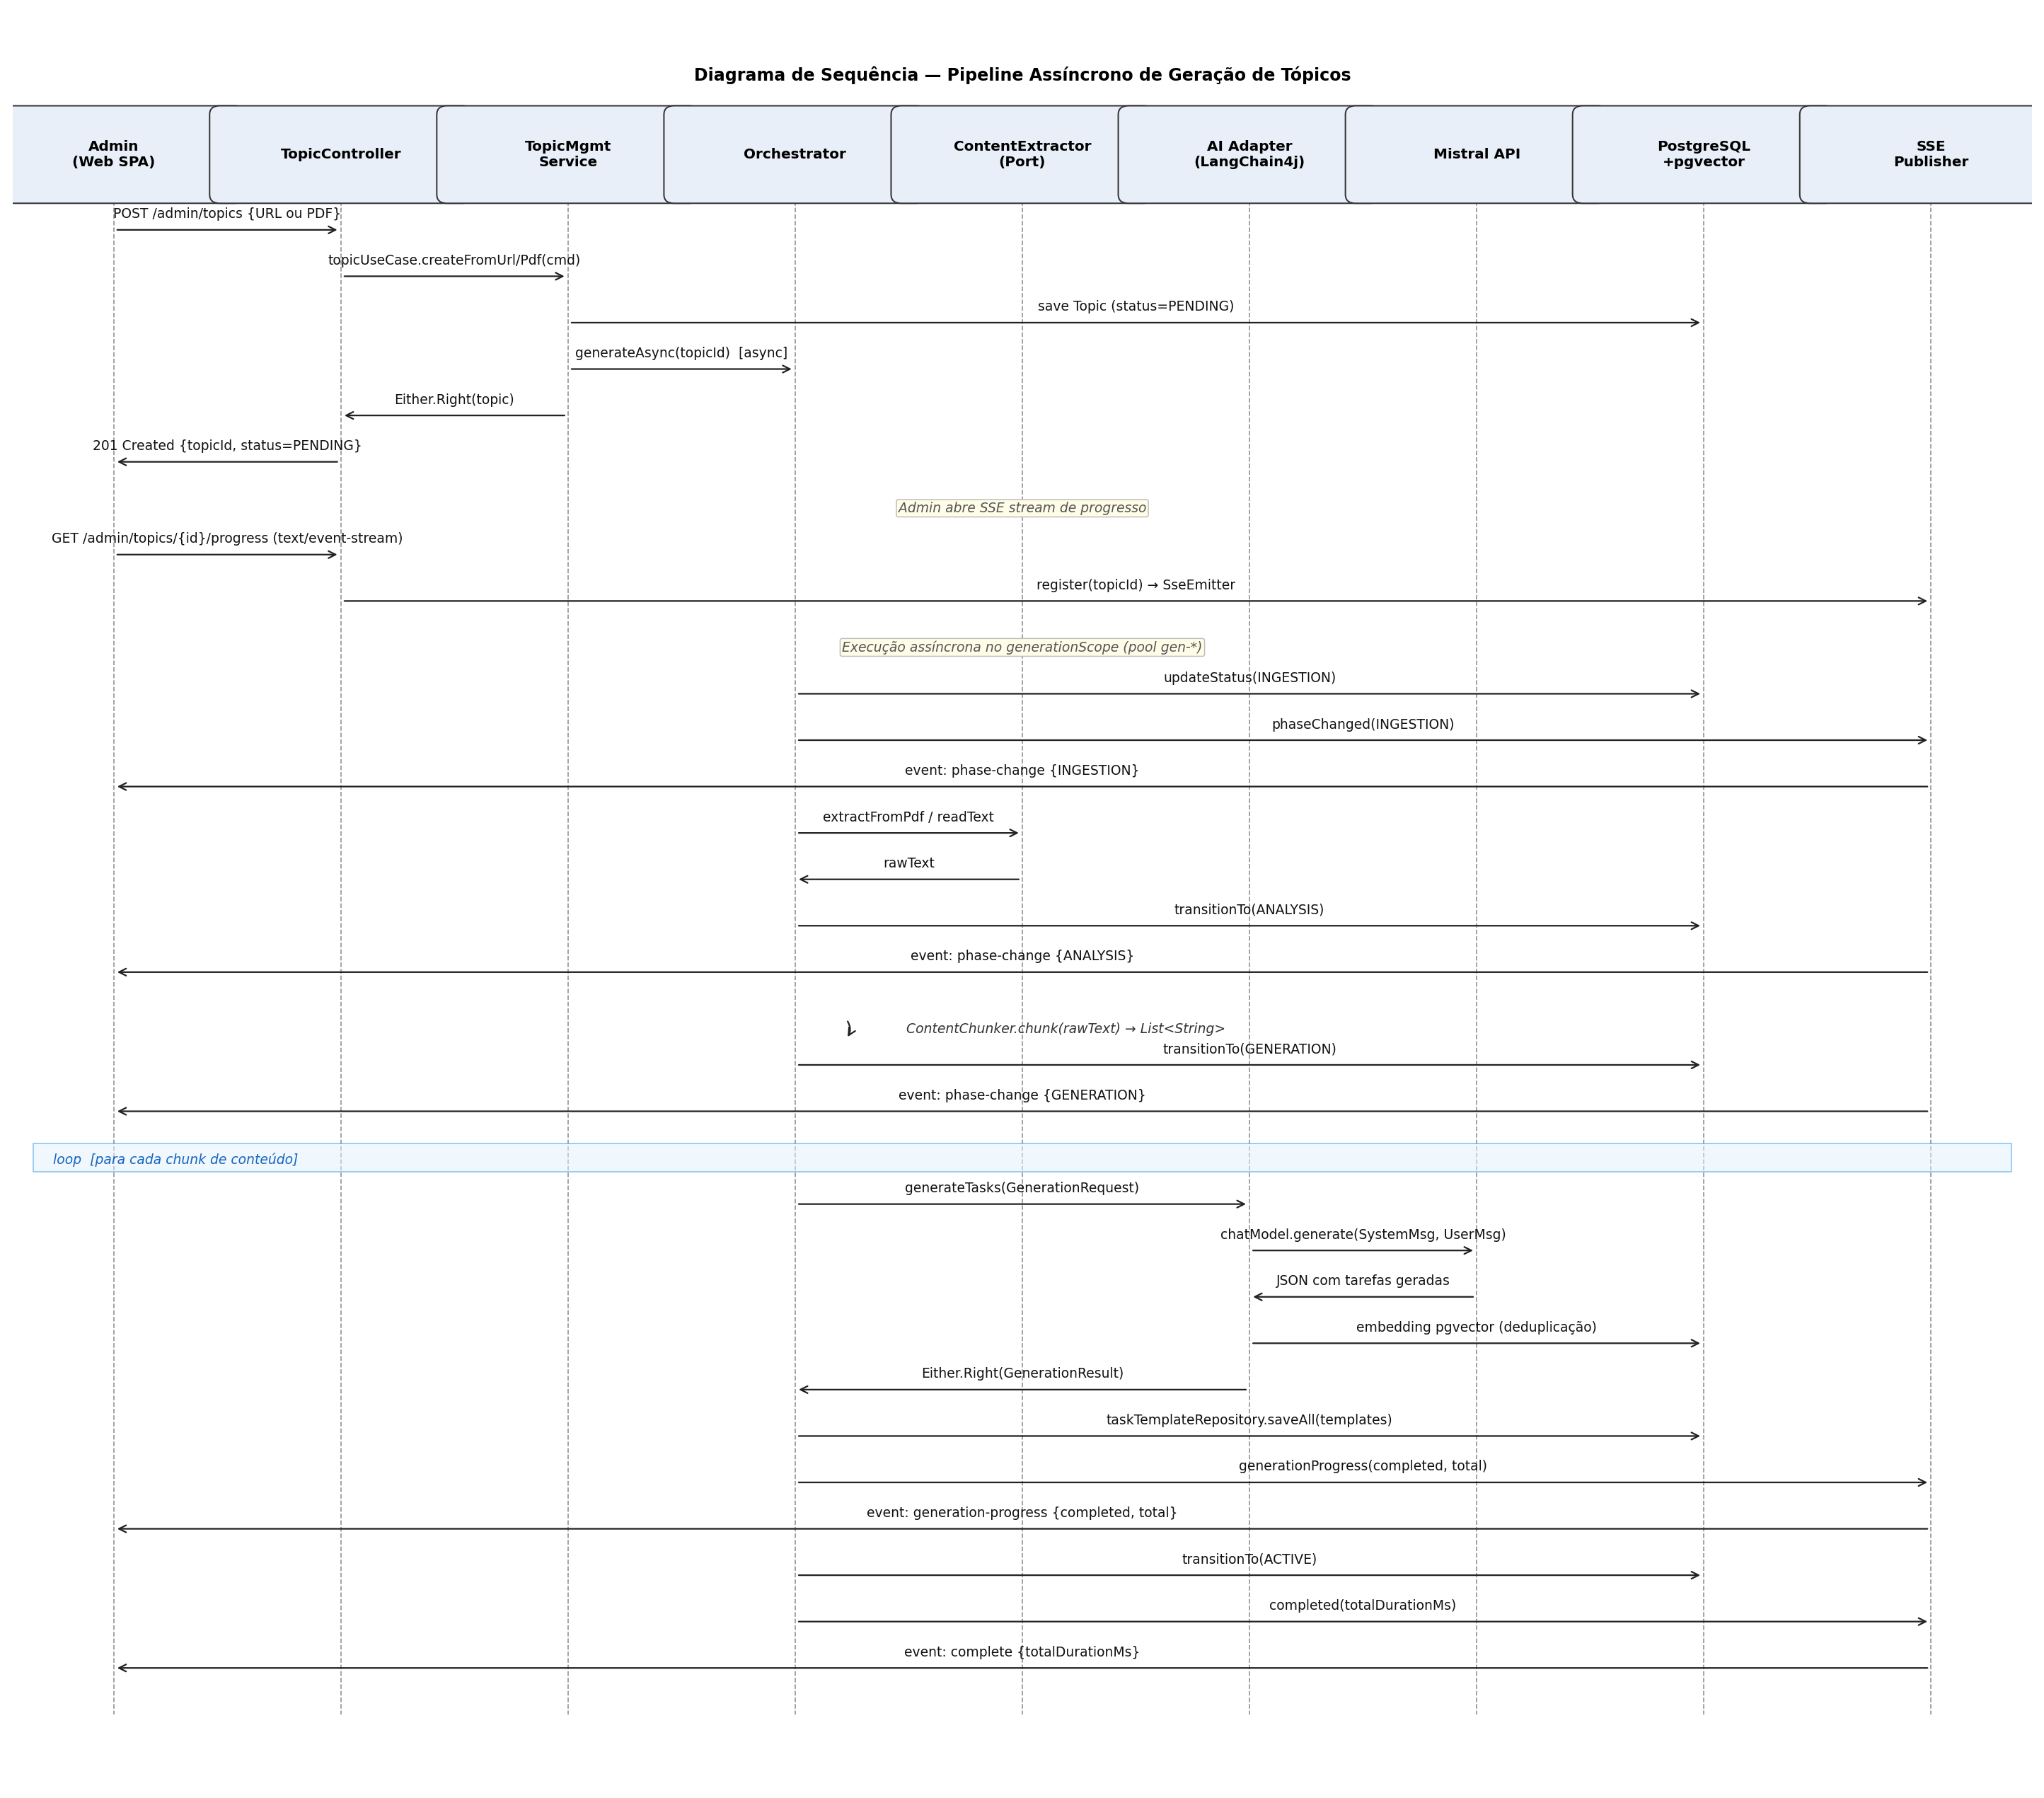
\includegraphics{./figures/seq-topic-generation.png}}
    \caption{Pipeline assíncrono de geração de tópicos com notificação SSE}
    \label{fig:seq-topic-gen}
\end{figure}

\subsection*{Autenticação por Magic Link}

Ilustra o fluxo completo de autenticação por \textit{magic link} descrito na Secção~\ref{sec:auth-flow} do Capítulo~\ref{cap:desenvolvimento}, incluindo os casos de token inválido, expirado ou já usado.

\begin{figure}[h!]
    \centering
    \resizebox{0.8\textwidth}{!}{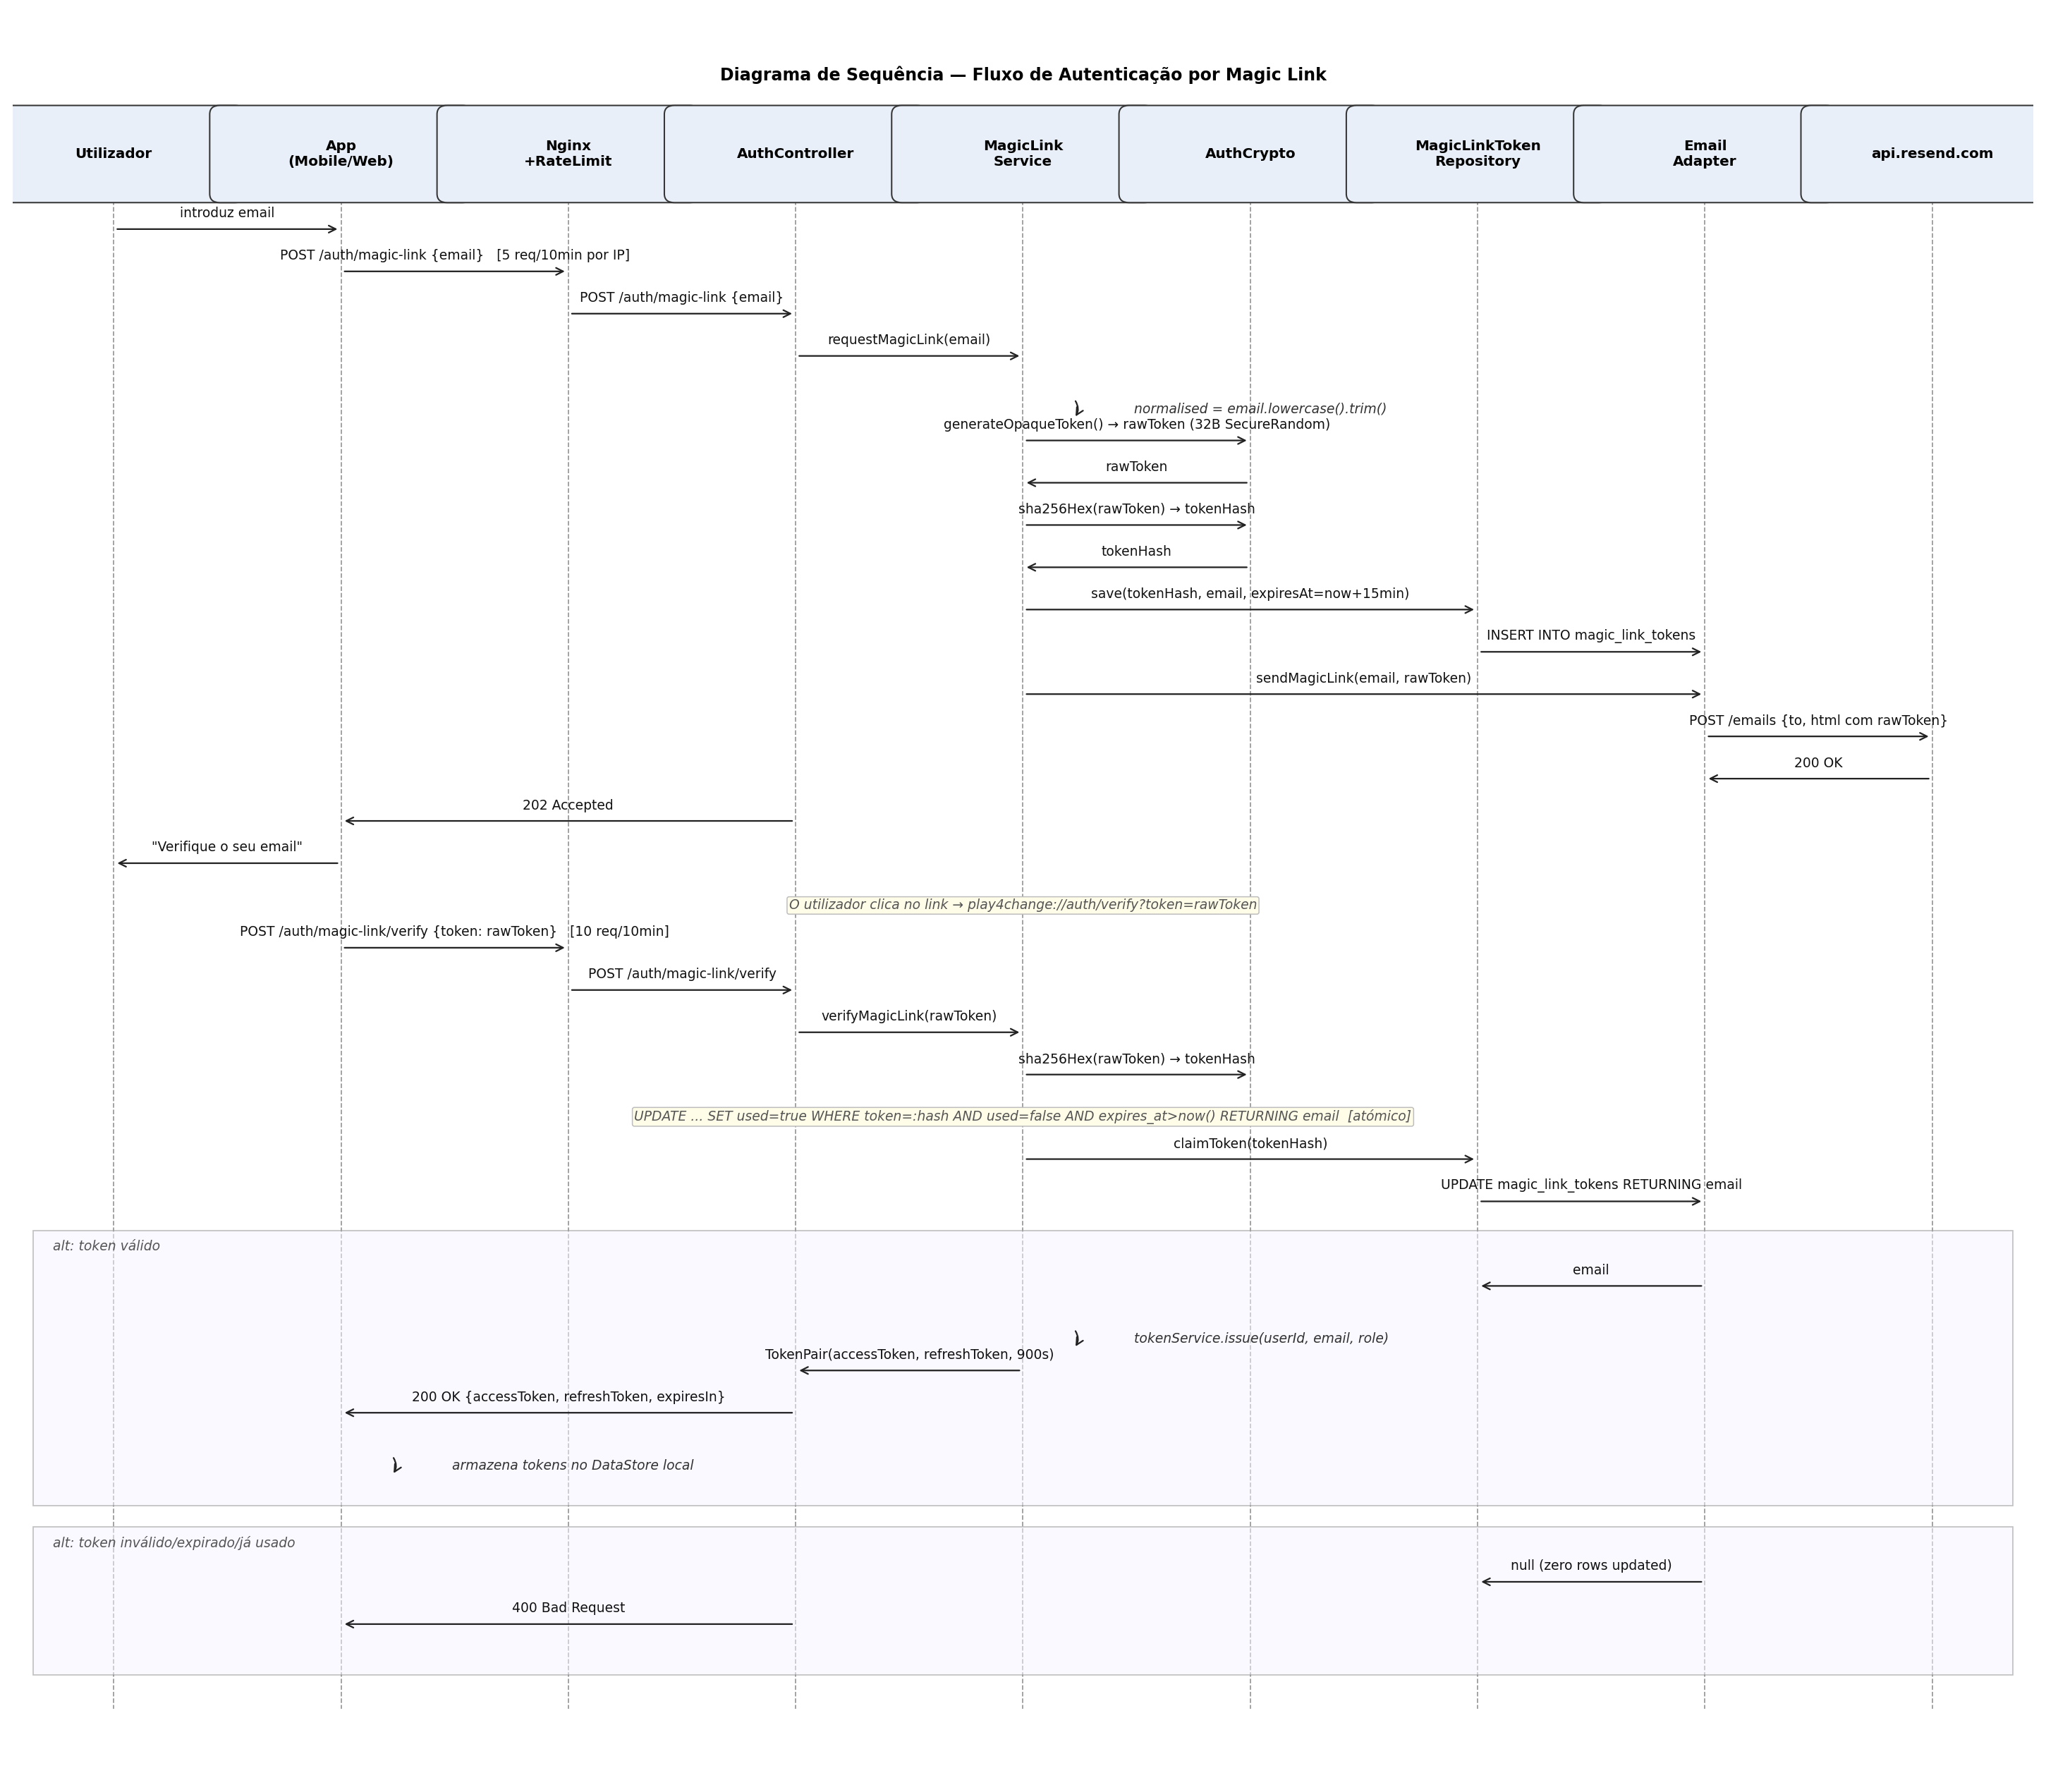
\includegraphics{./figures/seq-magic-link.png}}
    \caption{Diagrama de sequência --- fluxo completo de autenticação por \textit{magic link}}
    \label{fig:seq-magic-link}
\end{figure}

\subsection*{Extração de Texto de URL com Validação SSRF}

Ilustra o fluxo de ingestão por URL descrito na Secção~\ref{sec:url} do Capítulo~\ref{cap:ingestao}, incluindo a validação \texttt{UrlSsrfValidator} antes de qualquer pedido ao \textit{scraper} Playwright.

\begin{figure}[h!]
    \centering
    \resizebox{0.8\textwidth}{!}{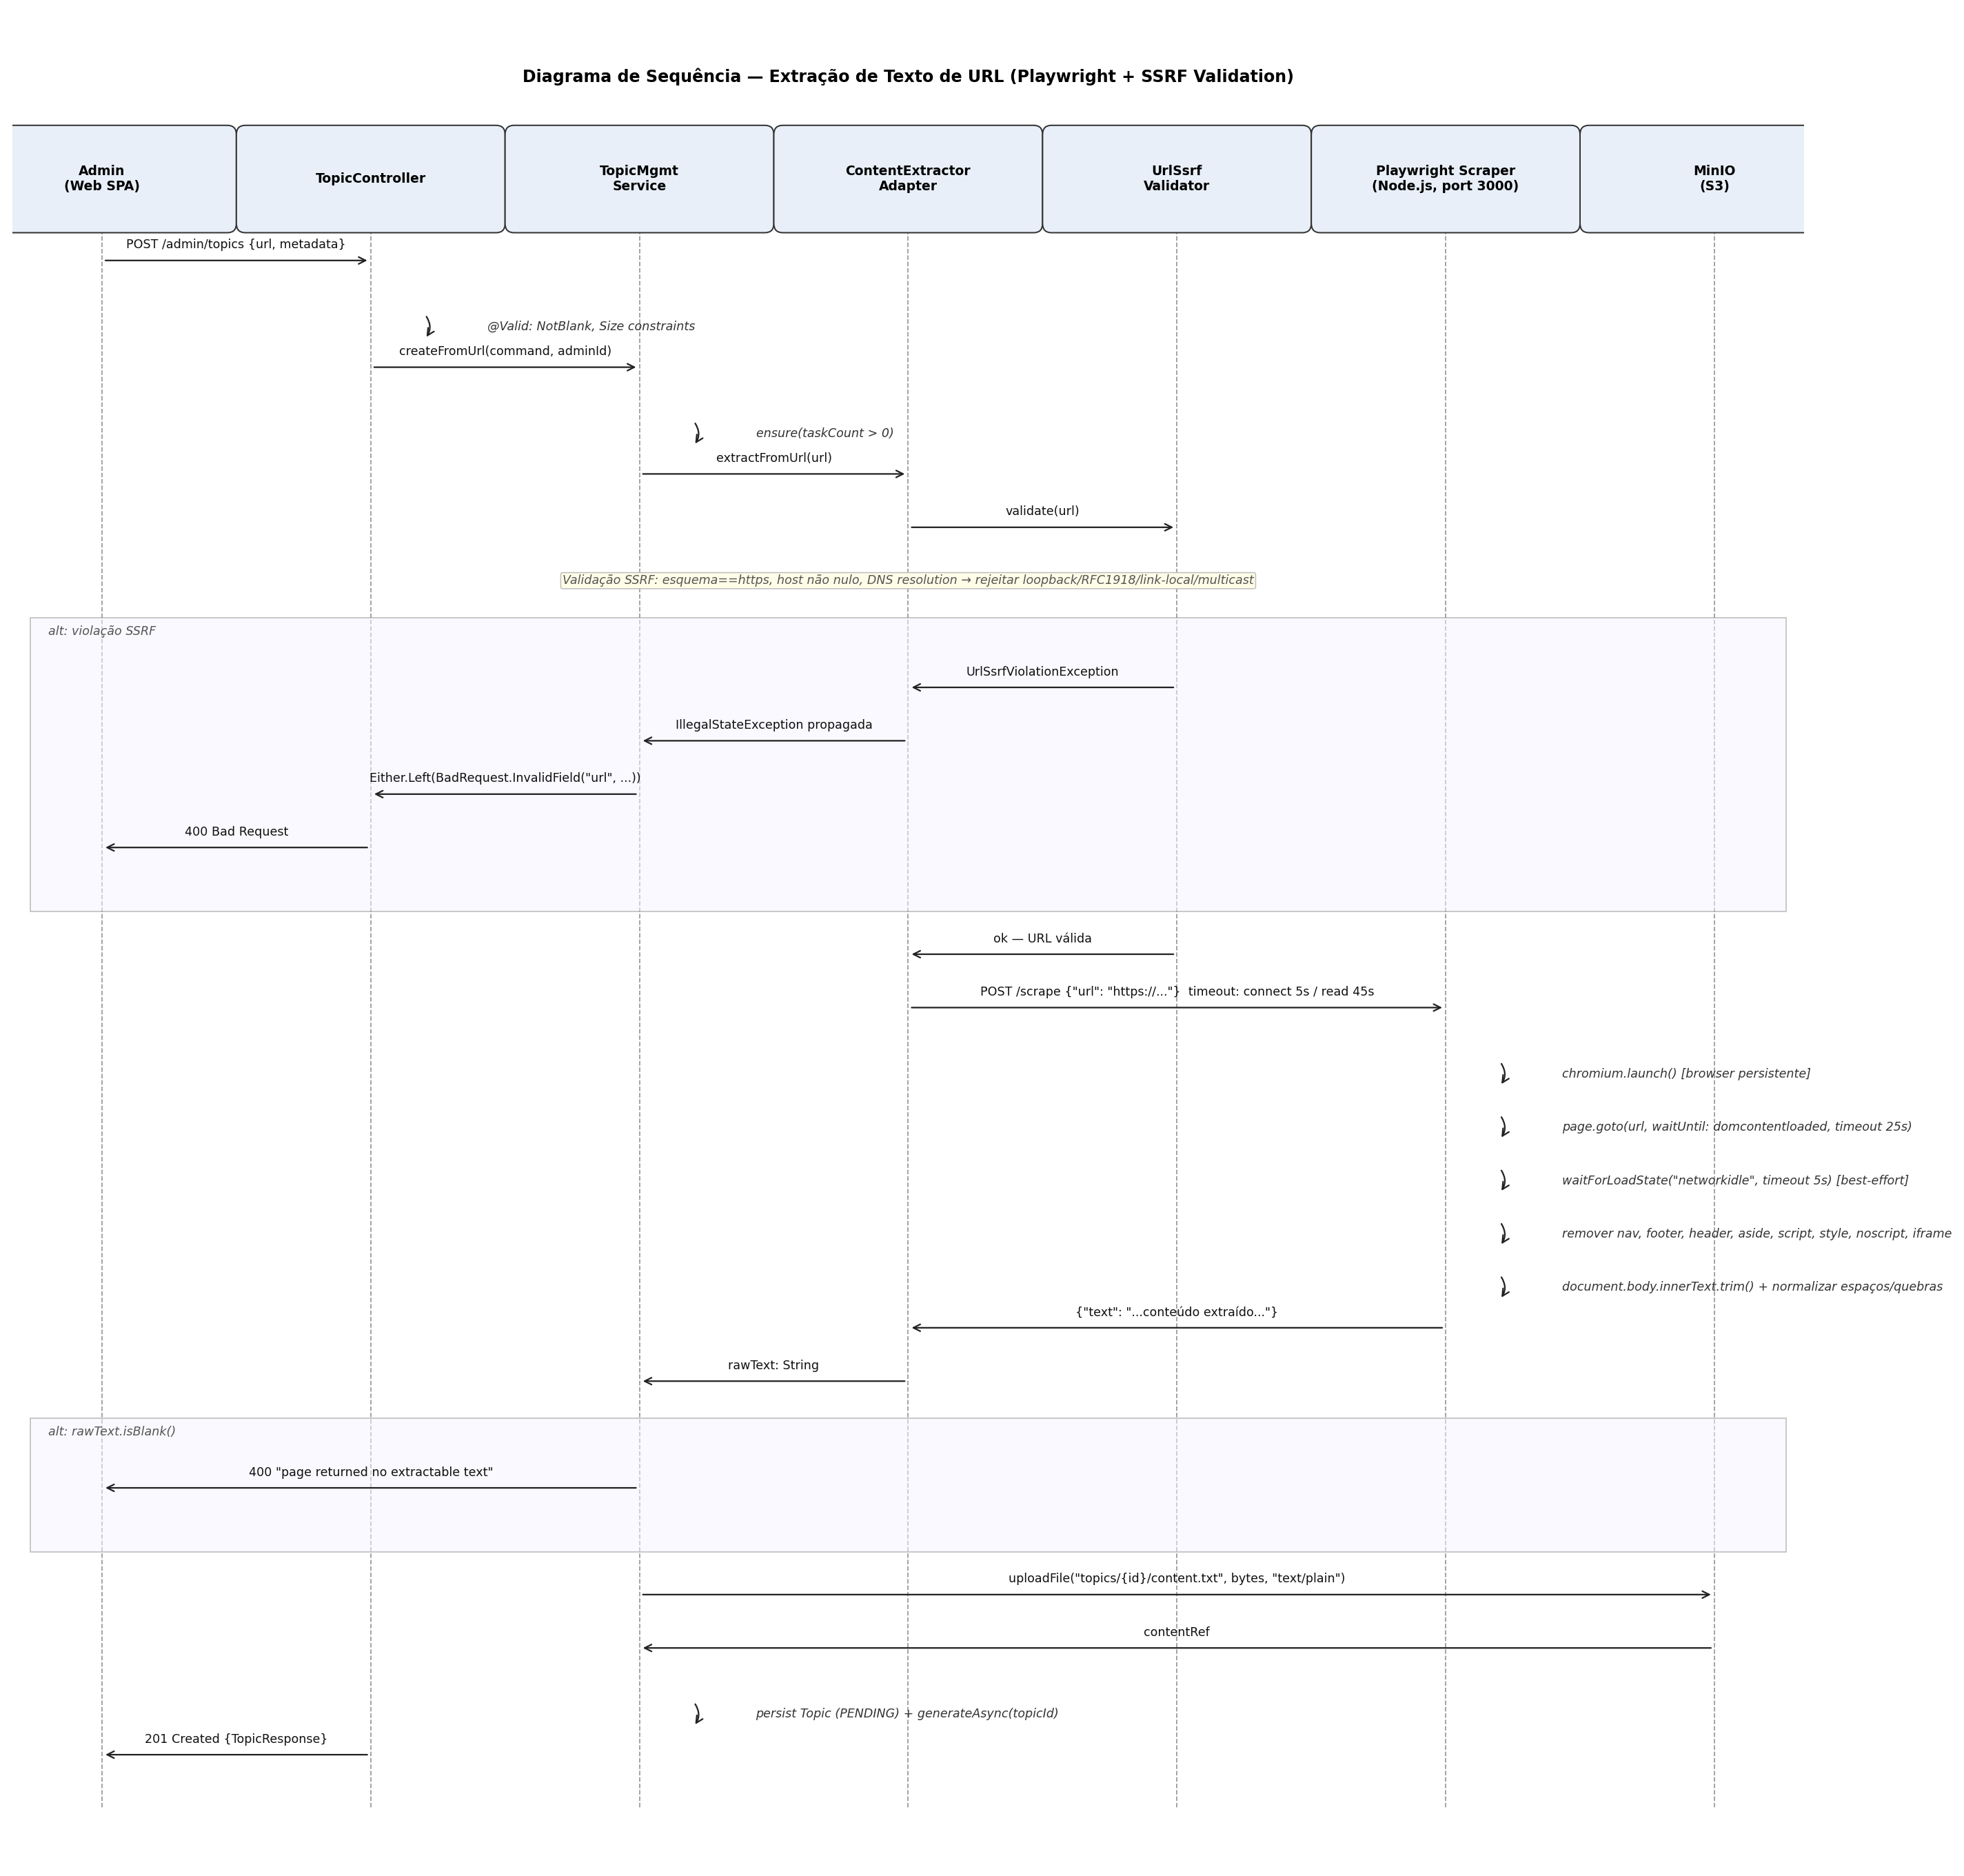
\includegraphics{./figures/seq-ingest-url.png}}
    \caption{Diagrama de sequência --- extração de texto de URL com validação SSRF e Playwright}
    \label{fig:seq-ingest-url}
\end{figure}

\subsection*{Arquitetura Anti-\textit{Prompt Injection}}

Ilustra a construção da lista de mensagens tipadas descrita na Secção~\ref{sec:protecao-ia} do Capítulo~\ref{cap:ia}, que isola o input do utilizador do \texttt{SystemMessage} de confiança.

\begin{figure}[h!]
    \centering
    \resizebox{0.8\textwidth}{!}{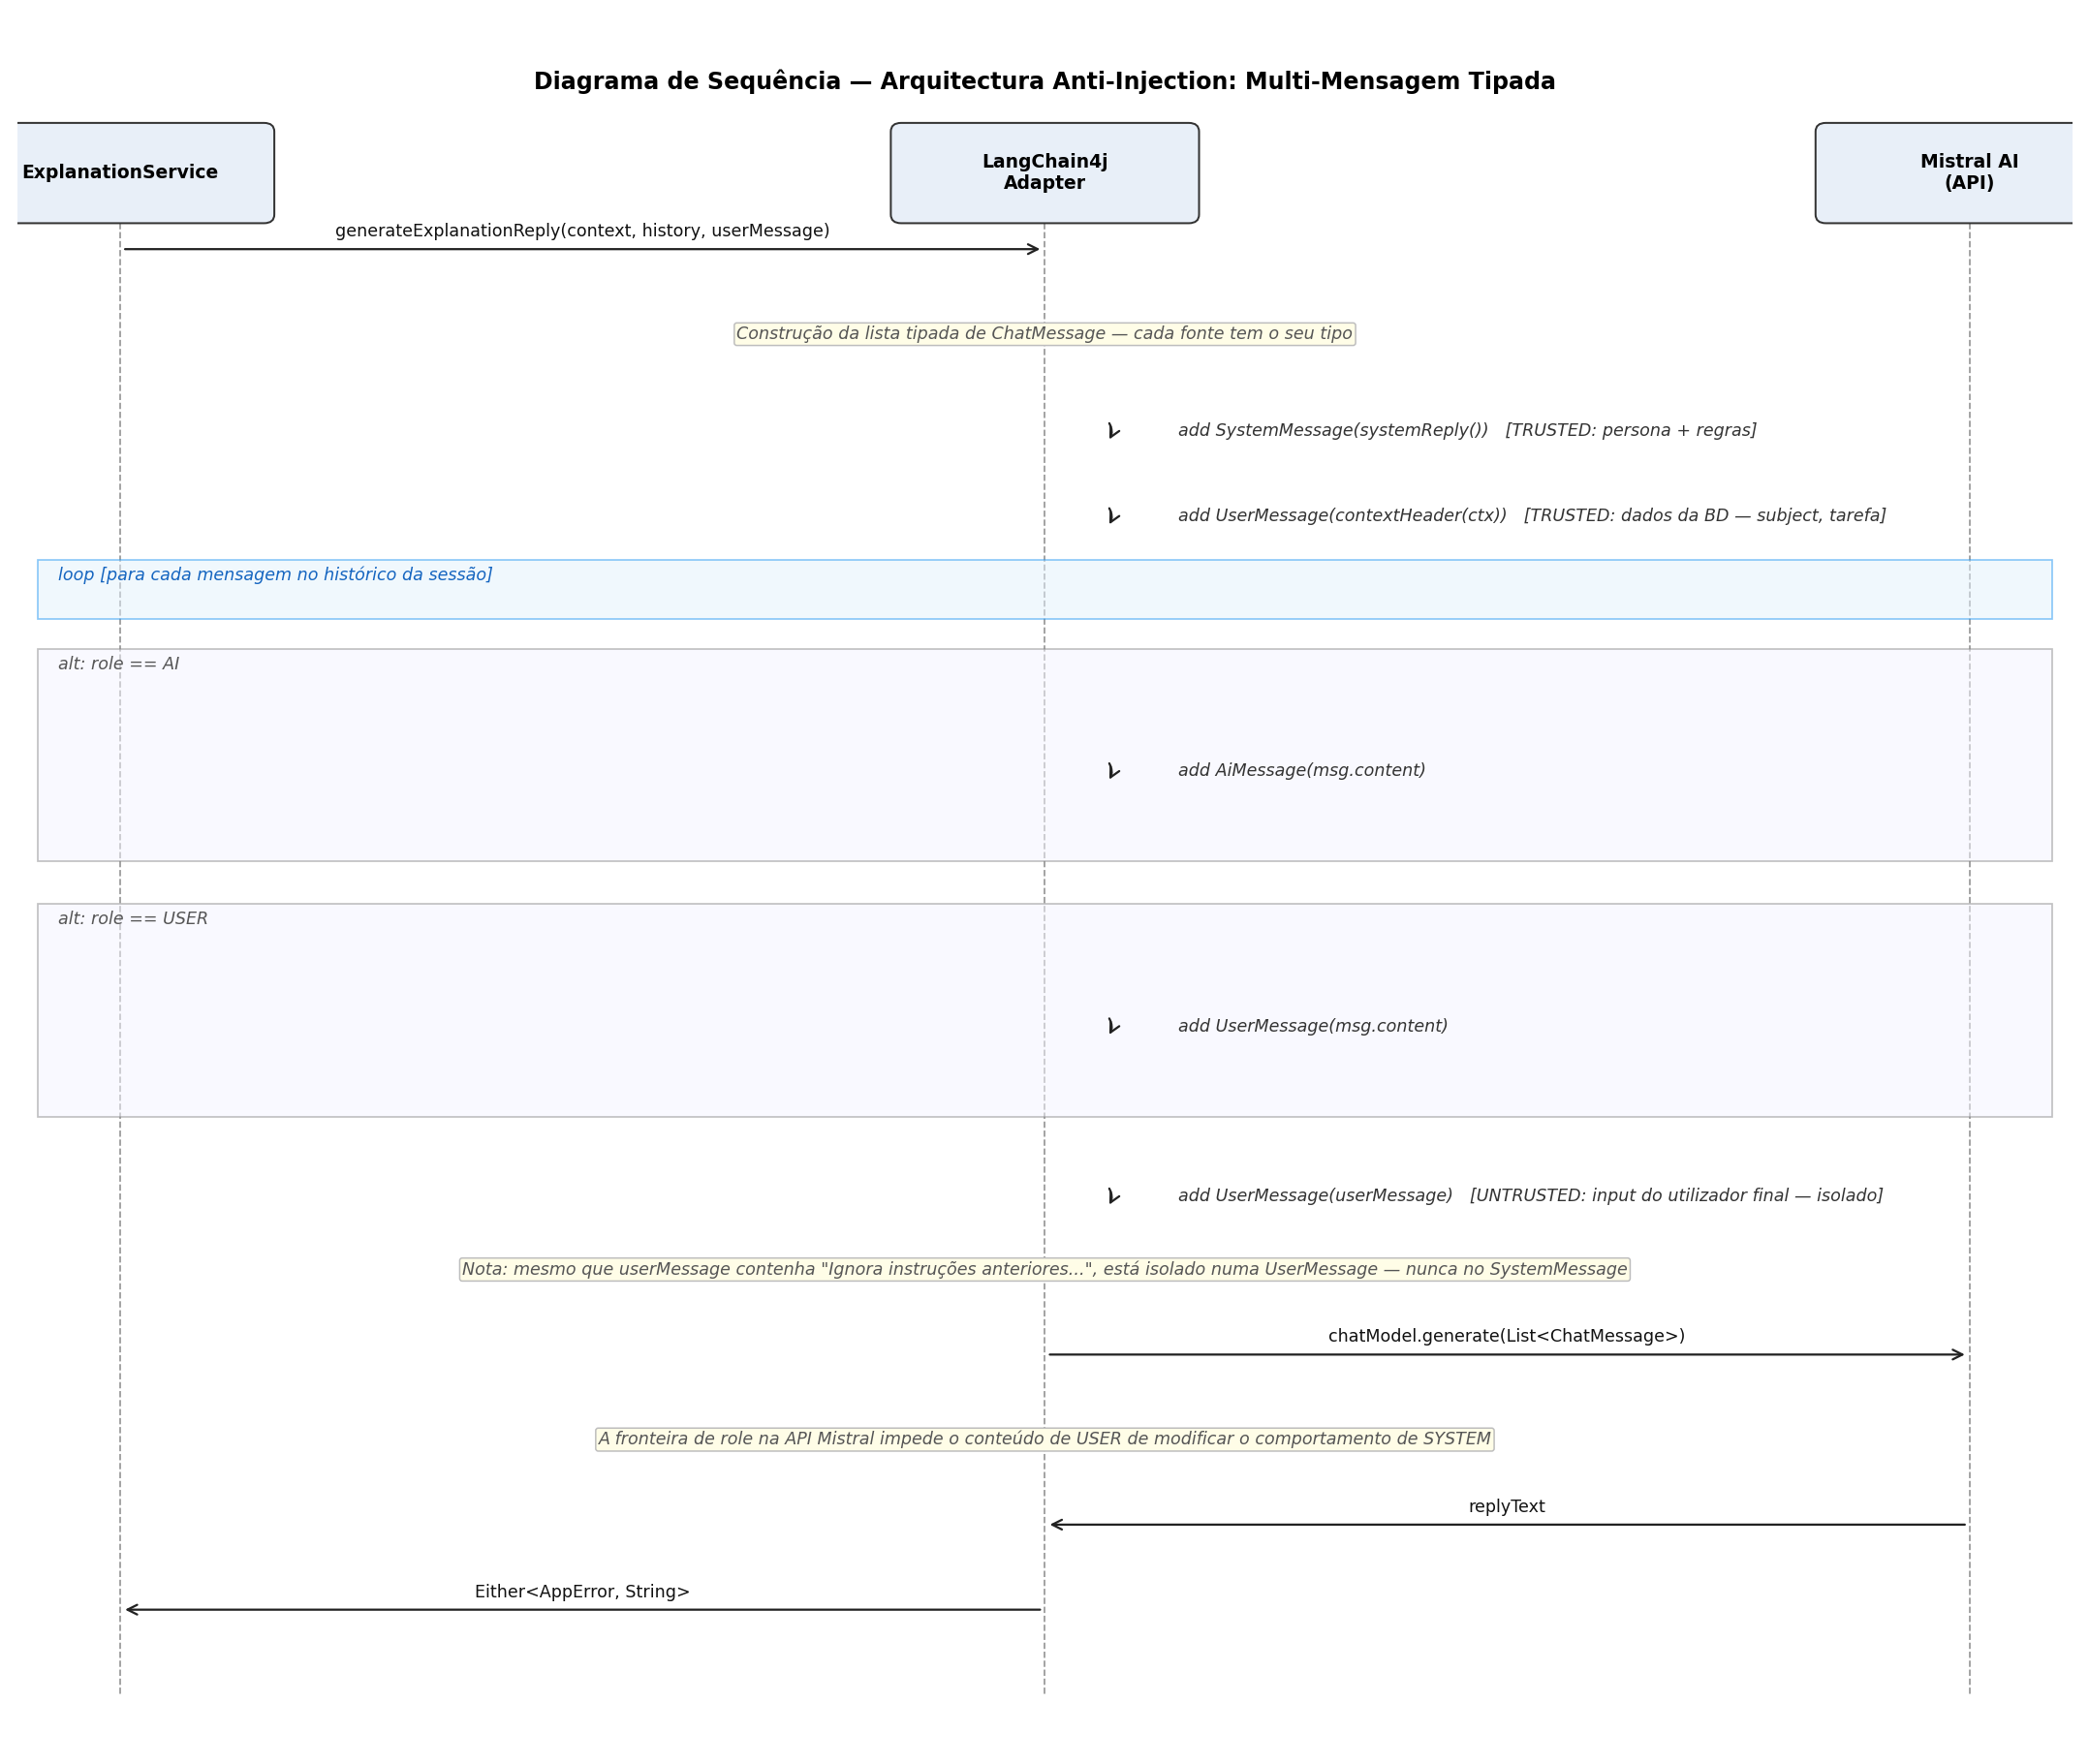
\includegraphics{./figures/seq-ai-anti-injection.png}}
    \caption{Arquitetura anti-\textit{injection}: construção tipada de mensagens por nível de confiança}
    \label{fig:seq-ai-anti-injection}
\end{figure}

\subsection*{Tutoria com IA}

Ilustra o fluxo da sessão de tutoria com IA descrito na Secção~\ref{sec:explicacao-ia} do Capítulo~\ref{cap:desafios}: geração holística assíncrona, diálogo conversacional multi-turno e resolução, usando a mesma estrutura de mensagens tipadas isolada acima.

\begin{figure}[h!]
    \centering
    \resizebox{0.8\textwidth}{!}{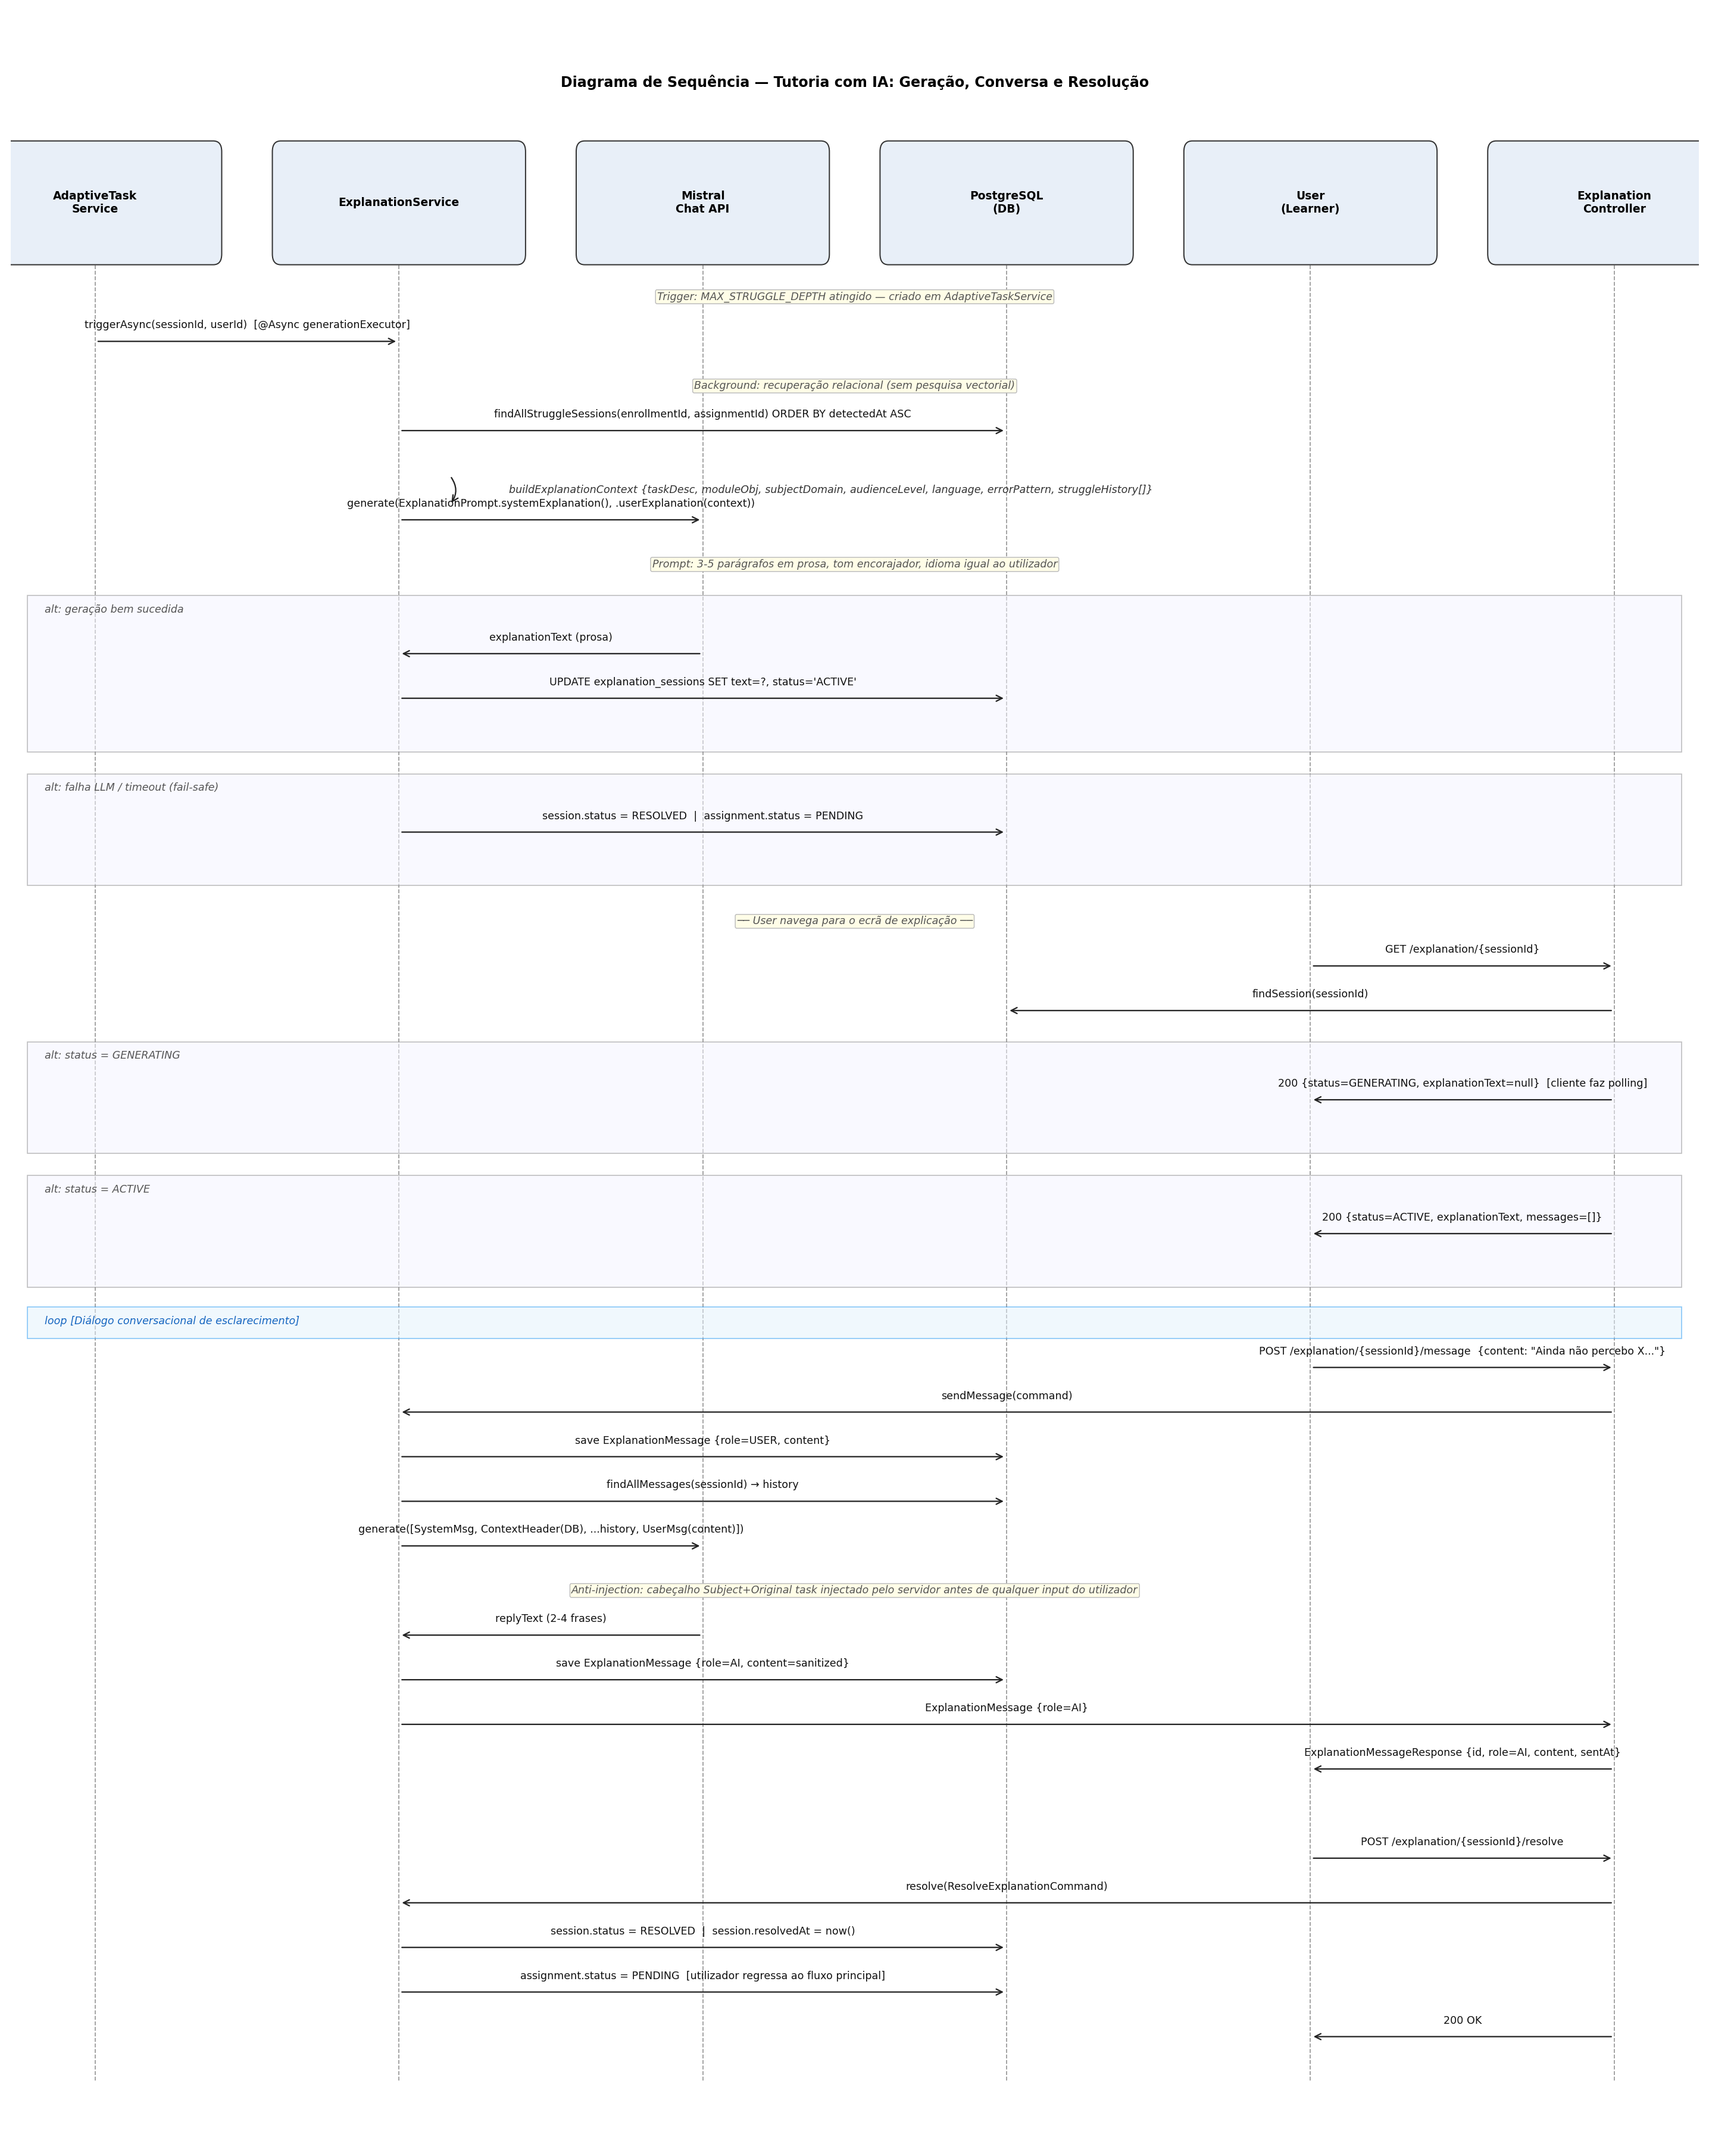
\includegraphics{./figures/seq-explanation-conv.png}}
    \caption{Tutoria com IA --- geração assíncrona, diálogo conversacional e resolução}
    \label{fig:seq-explanation-conv}
\end{figure}

\section{Modelo de Dados de Autenticação} \label{ap:auth-detalhe}

\subsection*{Geração de Tokens e Propriedades Criptográficas}

Todos os tokens são gerados pela classe \texttt{AuthCrypto} com 32 bytes de \texttt{SecureRandom} (64 caracteres hexadecimais). Apenas o \textit{hash} SHA-256 do token é persistido; o token em claro existe exclusivamente em memória e no email enviado ao utilizador, nunca na base de dados.

\begin{table}[h!]
\centering
\caption{Tabelas do modelo de dados de autenticação}
\label{tab:auth-schema}
\resizebox{\textwidth}{!}{%
\begin{tabular}{lp{5cm}p{7cm}}
\hline
\textbf{Tabela} & \textbf{Campos relevantes} & \textbf{Função e propriedades de segurança} \\
\hline
\texttt{users}
  & \texttt{id} (UUID), \texttt{email}, \texttt{provider} (\texttt{MAGIC\_LINK}), \texttt{role} (\texttt{USER|ADMIN})
  & Perfil de autenticação; email é normalizado (lowercase + trim) antes de qualquer operação \\
\texttt{magic\_link\_tokens}
  & \texttt{token} (SHA-256 do token em claro), \texttt{expires\_at} (+15\,min), \texttt{used} (bool)
  & Apenas o \textit{hash} é persistido; consumo atómico via \texttt{UPDATE ... RETURNING} elimina janelas TOCTOU \\
\texttt{refresh\_tokens}
  & \texttt{token\_hash} (SHA-256), \texttt{family\_id} (UUID), \texttt{expires\_at} (+7\,dias), \texttt{used} (bool)
  & \texttt{family\_id} agrupa todos os \textit{tokens} de uma sessão; deteção de reutilização revoga toda a família \\
\texttt{recovery\_emails}
  & \texttt{email}, \texttt{verified} (bool), \texttt{token\_hash}, \texttt{token\_expires\_at} (+24\,h)
  & Permite autenticação com email alternativo verificado; não cria utilizador duplicado \\
\hline
\end{tabular}%
}
\end{table}

\subsection*{Decisões de Segurança do Fluxo Magic Link}

O fluxo de autenticação por \textit{magic link} (Figura~\ref{fig:seq-magic-link}) assenta em três decisões deliberadas. Primeiro, o pedido do \textit{link} (utilizador submete o email, \texttt{MagicLinkService} normaliza-o e persiste o SHA-256) responde sempre \texttt{202 Accepted}, independentemente de o email existir --- não confirmando nem negando a sua existência, evitando enumeração de contas. Segundo, o consumo do token (móvel via \textit{deep link}; web via \textit{redirect} que não consome, apenas encaminha para o POST) é uma operação atómica \texttt{UPDATE ... WHERE used=false AND expires\_at>now() RETURNING email}, eliminando janelas de corrida. Terceiro, zero linhas devolvidas significa indistintamente token inválido, expirado ou já usado --- as três condições de falha são propositadamente indistinguíveis para o cliente, evitando \textit{oracle attacks}.

\subsection*{Assinatura e Ciclo de Vida dos Tokens JWT}

O \textit{access token} é um JWT assinado com HMAC-SHA-256, com a estrutura de \textit{claims} \texttt{\{sub, email, role, iat, exp\}}. O algoritmo é fixado explicitamente no código (\texttt{signWith(key, Jwts.SIG.HS256)}) em vez de deixado à seleção automática do jjwt, que escolheria HS512 para o segredo de 64+ caracteres exigido em produção --- uma inconsistência entre o algoritmo documentado e o efetivamente usado, identificada em revisão e corrigida ao fixar o algoritmo explicitamente. A chave de assinatura é validada em arranque pelo \texttt{JwtSecretStartupGuard}: em perfil \texttt{prod}, o arranque falha (\texttt{IllegalStateException}) se a chave tiver menos de 64 caracteres ou for igual ao valor de desenvolvimento por omissão; fora de \texttt{prod}, o uso desse valor por omissão gera apenas um aviso em log, sem impedir o arranque. A sessão Spring é \texttt{STATELESS} (\texttt{SessionCreationPolicy.STATELESS}) --- cada pedido é autenticado independentemente pelo \texttt{JwtAuthFilter}.

O mecanismo de rotação de \textit{refresh tokens} segue o padrão \textit{token rotation} com deteção de reutilização. Quando o cliente faz \texttt{POST /auth/refresh}, o \texttt{TokenService} localiza o \textit{refresh token} pelo hash. Se o token já foi marcado como \texttt{used}, é detetado um possível roubo de sessão: todos os tokens da mesma \texttt{family\_id} são imediatamente revogados, forçando o utilizador a re-autenticar. Em caso de token válido, o token atual é marcado como usado e é emitido um novo par, mantendo o mesmo \texttt{family\_id} --- o que garante que o \textit{logout} revoga toda a cadeia de rotação da sessão.

\begin{table}[h!]
\centering
\caption{Zonas de controlo de acesso configuradas no Spring Security}
\label{tab:access-zones}
\resizebox{\textwidth}{!}{%
\begin{tabular}{lp{7cm}l}
\hline
\textbf{Zona} & \textbf{Paths} & \textbf{Requisito} \\
\hline
Pública
  & \texttt{/auth/**}, \texttt{/api/stats/public}, \texttt{/error}, \texttt{/actuator/health}, \texttt{/actuator/prometheus}
  & Sem autenticação \\
Swagger
  & \texttt{/swagger-ui/**}, \texttt{/v3/api-docs/**}
  & \texttt{ROLE\_ADMIN} em \textit{prod}; público em dev \\
Administração
  & \texttt{/admin/**}
  & \texttt{ROLE\_ADMIN} obrigatório \\
Utilizador
  & Todos os restantes \textit{paths}
  & JWT válido (qualquer \textit{role}) \\
\hline
\end{tabular}%
}
\end{table}

\section{Modelo de Dados de Desafios e Progressão}

\begin{table}[h!]
\centering
\caption{Campos de \texttt{TaskTemplate} e \texttt{TaskInstance}}
\label{tab:model-tasks}
\begin{tabular}{llp{8.5cm}}
\hline
\textbf{Entidade} & \textbf{Campo} & \textbf{Descrição} \\
\hline
\texttt{TaskTemplate} & \texttt{title}, \texttt{description}, \texttt{hint} & Conteúdo textual gerado pelo LLM \\
 & \texttt{taskType} & \texttt{MULTIPLE\_CHOICE}, único valor suportado \\
 & \texttt{options[4]}, \texttt{correctAnswer} & Quatro opções; resposta correta sempre no índice~0 \\
 & \texttt{embedding} & Vector de 1024 dimensões, usado para deduplicação \\
 & \texttt{dayIndex}, \texttt{poolIndex} & Posição no percurso e no conjunto de variantes \\
 & \texttt{version}, \texttt{isCurrent} & Controlo de versão para edição e regeneração \\
\hline
\texttt{TaskInstance} & \texttt{correctAnswer} & Partilhado com o \textit{template} de origem \\
 & \texttt{options} & Distratores alternativos, distintos por instância \\
 & (relação) & 1:N com \texttt{TaskTemplate}, até \texttt{instancesPerTask = 5} \\
\hline
\end{tabular}
\end{table}

\begin{table}[h!]
\centering
\caption{Campos de \texttt{Enrollment} e \texttt{TaskAssignment}}
\label{tab:model-assignment}
\begin{tabular}{llp{8.5cm}}
\hline
\textbf{Entidade} & \textbf{Campo} & \textbf{Descrição} \\
\hline
\texttt{Enrollment} & \texttt{currentDayIndex} & Dia corrente do percurso do utilizador no módulo \\
 & \texttt{status} & \texttt{ACTIVE} \textbar\ \texttt{COMPLETED} \textbar\ \texttt{EXPIRED} \textbar\ \texttt{PAUSED} \\
 & \texttt{totalPointsEarned}, \texttt{streakDays} & Pontuação e sequência de dias consecutivos \\
\hline
\texttt{TaskAssignment} & \texttt{enrollmentId}, \texttt{taskTemplateId}, \texttt{taskInstanceId} & Referências à inscrição, ao \textit{template} e à variante seleccionada \\
 & \texttt{optionOrder}, \texttt{correctAnswerIndex} & Permutação de opções apresentada e índice correto \\
 & \texttt{dueAt} & 24~horas após \texttt{assignedAt} \\
 & \texttt{status} & \texttt{PENDING} \textbar\ \texttt{SUBMITTED} \textbar\ \texttt{LATE} \\
 & \texttt{wrongAttemptCount} & Contador de tentativas erradas \\
\hline
\end{tabular}
\end{table}

\section{Campos do Pedido de Ingestão por PDF}

\begin{table}[h!]
\centering
\caption{Campos do pedido \texttt{POST /admin/topics/pdf} (multipart/form-data)}
\label{tab:pdf-fields}
\resizebox{\textwidth}{!}{%
\begin{tabular}{llll}
\hline
\textbf{Campo} & \textbf{Tipo} & \textbf{Obrigatório} & \textbf{Restrições} \\
\hline
\texttt{file}        & binary PDF  & Sim & máx.\ 25\,MB \\
\texttt{title}       & String      & Sim & máx.\ 200 caracteres \\
\texttt{description} & String      & Sim & máx.\ 1\,000 caracteres \\
\texttt{category}    & String      & Não & máx.\ 100 caracteres \\
\texttt{difficulty}  & Enum        & Não & \texttt{BEGINNER | INTERMEDIATE | ADVANCED} (omissão: \texttt{BEGINNER}) \\
\texttt{language}    & String      & Não & código ISO 639-1 (omissão: \texttt{en}), máx.\ 10 caracteres \\
\texttt{taskCount}   & Int         & Não & omissão: 10 \\
\texttt{expiresAt}   & ISO 8601    & Não & omissão: agora + 90 dias \\
\hline
\end{tabular}%
}
\end{table}

O fluxo por URL (\texttt{POST /admin/topics}) partilha o mesmo esquema, substituindo \texttt{file} por \texttt{url} (String, sujeito a validação SSRF --- Capítulo~\ref{cap:ingestao}).

\section{Cenários de Falha na Extração de Conteúdo}

\begin{table}[h!]
\centering
\caption{Cenários de falha na extração de conteúdo e respostas HTTP}
\label{tab:ingest-errors}
\resizebox{\textwidth}{!}{%
\begin{tabular}{lll}
\hline
\textbf{Cenário} & \textbf{Resposta} & \textbf{Campo em erro} \\
\hline
PDF com apenas imagens sem OCR bem-sucedida   & \texttt{400} ``PDF contains no extractable text''     & \texttt{file} \\
Página com conteúdo exclusivamente em canvas  & \texttt{400} ``page returned no extractable text''    & \texttt{url}  \\
Timeout ou indisponibilidade do Unstructured  & \texttt{400} com mensagem de erro propagada           & \texttt{file} \\
Timeout ou indisponibilidade do scraper       & \texttt{400} com mensagem de erro propagada           & \texttt{url}  \\
Violação SSRF                                 & \texttt{400} com detalhe da violação                  & \texttt{url}  \\
\hline
\end{tabular}%
}
\end{table}

\section{Casos de Teste de Prevenção de SSRF}

O vetor SSRF é crítico porque os administradores submetem URLs de conteúdo que a aplicação vai buscar para gerar tarefas com IA (Capítulo~\ref{cap:ingestao}). O \texttt{UrlSsrfValidatorTest.kt} (10 testes, referido na Secção~\ref{sec:estrategia-testes} do Capítulo~\ref{cap:testes}) valida que \texttt{UrlSsrfValidator.validate()} lança \texttt{UrlSsrfViolationException} para cada categoria de URL proibida, detalhada na Tabela~\ref{tab:ssrf-casos}.

\begin{table}[h!]
\centering
\caption{Casos de teste de prevenção de SSRF — \texttt{UrlSsrfValidatorTest}.}
\label{tab:ssrf-casos}
\begin{tabular}{@{}p{6cm}p{4cm}p{4.3cm}@{}}
\toprule
\textbf{URL testada} & \textbf{Categoria} & \textbf{Resultado} \\
\midrule
\texttt{https://localhost/admin}, \texttt{127.0.0.1}, \texttt{[::1]} & Loopback (IPv4/IPv6) & \texttt{Url\allowbreak Ssrf\allowbreak Violation\allowbreak Exception} \\
\texttt{192.168.1.1}, \texttt{10.0.0.1}, \texttt{172.16.0.1}     & RFC~1918 (redes privadas) & \texttt{Url\allowbreak Ssrf\allowbreak Violation\allowbreak Exception} \\
\texttt{https://169.254.1.1/metadata}    & Link-local            & \texttt{Url\allowbreak Ssrf\allowbreak Violation\allowbreak Exception} \\
\texttt{http://example.com/page}         & Esquema HTTP (não HTTPS) & \texttt{Url\allowbreak Ssrf\allowbreak Violation\allowbreak Exception} \\
\texttt{https://nonexistent.tld.invalid} & Host inexistente (DNS falha) & \texttt{Url\allowbreak Ssrf\allowbreak Violation\allowbreak Exception} \\
\texttt{https://1.1.1.1/}               & IP público conhecido  & Sem exceção \\
\bottomrule
\end{tabular}
\end{table}

\section{Headers HTTP de Segurança (Nginx)}

\begin{table}[h!]
\centering
\caption{Headers HTTP de segurança configurados no Nginx (incl. diretivas CSP)}
\label{tab:security-headers}
\resizebox{\textwidth}{!}{%
\begin{tabular}{lll}
\hline
\textbf{Header} & \textbf{Valor} & \textbf{Proteção} \\
\hline
\texttt{Strict-Transport-Security} & \texttt{max-age=63072000; includeSubDomains} & Força HTTPS por 2 anos, inclui subdomínios \\
\texttt{X-Content-Type-Options}    & \texttt{nosniff}                             & Impede MIME-type \textit{sniffing} \\
\texttt{X-Frame-Options}           & \texttt{DENY}                                & Previne \textit{clickjacking} \\
\texttt{Referrer-Policy}           & \texttt{strict-origin-when-cross-origin}     & Limita informação de \textit{referrer cross-origin} \\
\texttt{Content-Security-Policy}\textsuperscript{*} & \texttt{default-src/script-src 'self'; style-src 'self' 'unsafe-inline'; img-src 'self' data:; connect-src 'self'; frame-ancestors 'none'} & Previne XSS e \textit{clickjacking} via política de \textit{browser} \\
\hline
\end{tabular}%
}
\end{table}
\textsuperscript{*}Ao contrário dos restantes \textit{headers} desta tabela, aplicados globalmente, a CSP está configurada apenas no bloco \texttt{location /} do \texttt{nginx.conf} (SPA estática), não nas rotas de API proxied.

\section{Catálogo de Métricas Instrumentadas}

\begin{table}[htb]
\centering
\caption{Catálogo de métricas instrumentadas com Micrometer.}
\label{tab:metricas-app}
\resizebox{\textwidth}{!}{%
\begin{tabular}{@{}llll@{}}
\toprule
\textbf{Métrica} & \textbf{Tipo} & \textbf{Tags} & \textbf{Descrição} \\
\midrule
\texttt{http\_server\_requests\_seconds}        & Timer   & uri, method, status                                 & Latência e throughput HTTP (Spring MVC auto) \\
\texttt{task.generation.duration}               & Timer   & status (success/failed/timeout)                     & Duração total da pipeline de geração por tópico \\
\texttt{ai.generation.duration}                 & Timer   & generation\_phase (GENERATION/ANALYSIS)             & Tempo de chamada ao Mistral por fase \\
\texttt{ai.generation.failures}                 & Counter & type                                                & Falhas de geração por categoria \\
\texttt{ai.adaptive.reuse}                      & Counter & strategy (full/partial/fresh)                       & Distribuição de estratégias de reutilização \\
\texttt{ai.dedup.duplicates\_skipped}           & Counter & module\_id                                          & Tarefas descartadas por deduplicação semântica \\
\texttt{ai.struggle.reuse\_strategy}            & Counter & strategy                                            & Estratégia de reuso no pgvector por ocorrência \\
\texttt{struggle\_sessions\_total}              & Counter & error\_pattern                                      & Sessões de dificuldade por padrão de erro \\
\texttt{explanation\_sessions\_created\_total}  & Counter & —                                                   & Total de sessões de explicação criadas \\
\texttt{explanation\_sessions\_resolved\_total} & Counter & outcome                                             & Resultado das sessões de explicação \\
\texttt{task\_submissions\_total}               & Counter & outcome (correct/incorrect/late), task\_type        & Submissões por resultado e tipo de tarefa \\
\texttt{tasks\_submitted\_total}                & Counter & result (correct/incorrect), topic\_id               & Submissões por resultado e tópico (métrica complementar orientada a análise por tópico) \\
\texttt{enrollments\_completed\_total}          & Counter & topic\_id                                           & Inscrições concluídas por tópico \\
\texttt{topic\_enrollments\_total}              & Counter & topic\_id                                           & Inscrições iniciadas por tópico \\
\texttt{struggle\_sessions\_created\_total}     & Counter & topic\_id                                           & Sessões de dificuldade criadas, por tópico \\
\texttt{struggle\_sessions\_escalated\_to\_explanation\_total} & Counter & --                                     & Sessões de dificuldade escaladas para tutoria com IA \\
\texttt{rate\_limit\_exceeded\_total}           & Counter & path                                                & Bloqueios por limite de taxa por caminho de API \\
\texttt{executor\_queued\_tasks}                & Gauge   & name=generationExecutor                             & Tarefas na fila do thread pool de geração \\
\texttt{jvm\_memory\_used\_bytes}               & Gauge   & area=heap/nonheap                                   & Utilização de memória JVM \\
\texttt{resilience4j\_circuitbreaker\_state}    & Gauge   & name=aiAgent, state                                 & Estado do circuit breaker de IA (aiAgent) \\
\bottomrule
\end{tabular}%
}
\end{table}

Note-se que \texttt{executor\_queued\_tasks} depende do \textit{binder} automático do Spring Boot para \texttt{ThreadPoolTaskExecutor} (introduzido na série 3.2); ao contrário das restantes métricas desta tabela, não existe nenhuma linha de código que registe explicitamente este nome --- pelo que a sua disponibilidade efetiva sob esse nome exato não foi confirmada em runtime e deve ser validada antes de se confiar no alerta \texttt{GenerationThreadPoolQueueSaturated} (Tabela~\ref{tab:alertas}) que a consome.

\section{Regras de Alerta Prometheus}

\begin{table}[htb]
\centering
\caption{Regras de alerta Prometheus configuradas (\textit{evaluation\_interval}: 15s).}
\label{tab:alertas}
\resizebox{\textwidth}{!}{%
\begin{tabular}{@{}lllll@{}}
\toprule
\textbf{Alerta} & \textbf{Expressão PromQL (simplificada)} & \textbf{Limiar} & \textbf{Duração} & \textbf{Sev.} \\
\midrule
ServerDown                         & \texttt{up\{job="spring-boot"\} == 0}                               & —      & 1~min  & Crítico \\
AiCircuitBreakerOpen               & \texttt{resilience4j\_circuitbreaker\_state\{state="open"\} == 1}   & —      & Imediato & Crítico \\
JvmHeapUsageCritical               & \texttt{jvm\_memory\_used / jvm\_memory\_max}                        & > 95\% & 2~min  & Crítico \\
HighHttpErrorRate                  & \texttt{rate(http\_5xx[5m]) / rate(http\_all[5m])}                  & > 5\%  & 2~min  & Aviso \\
HighAiGenerationFailureRate        & \texttt{rate(ai\_generation\_failures\_total[10m])}                  & > 0,1/s & 5~min & Aviso \\
AiGenerationP95High                & \texttt{histogram\_quantile(0.95, task.generation[10m])}             & > 90~s & 5~min  & Aviso \\
JvmHeapUsageHigh                   & \texttt{jvm\_memory\_used / jvm\_memory\_max}                        & > 85\% & 5~min  & Aviso \\
GenerationThreadPoolQueueSaturated & \texttt{executor\_queued\_tasks\{name="generationExecutor"\}}        & $\geq$ 20 & 2~min & Aviso \\
\bottomrule
\end{tabular}%
}
\end{table}

%
% Apêndice D — Garantias de Qualidade e Configuração Operacional
%
\chapter{Garantias de Qualidade e Configuração Operacional} \label{ap:qualidade-config}

Este apêndice reúne, num único local, as garantias de qualidade aplicadas a cada questão gerada por Inteligência Artificial e os parâmetros de configuração operacional referenciados a partir dos Capítulos~\ref{cap:intro}, \ref{cap:desenvolvimento}, \ref{cap:ingestao}, \ref{cap:ia}, \ref{cap:geracao-desafios}, \ref{cap:seguranca} e \ref{cap:discussao}.

\section{Garantias de Qualidade das Questões Geradas}

\begin{table}[h!]
\centering
\caption{Garantias de qualidade das questões geradas}
\label{tab:garantias-qualidade}
\begin{tabular}{cp{10.5cm}}
\hline
\textbf{Nº} & \textbf{Garantia} \\
\hline
1 & \textbf{Unicidade semântica} --- similaridade coseno $< 0{,}90$ com qualquer tarefa já existente no mesmo módulo, verificada por consulta pgvector (índice IVFFlat) sobre o \textit{embedding} de 1024 dimensões do \texttt{TaskTemplate} (§\ref{sec:armazenamento}). \\
2 & \textbf{Formato válido} --- o esquema JSON imposto ao modelo exige exatamente 4 opções por questão; a resposta correta é sempre persistida no índice~0 e só é baralhada no momento de apresentação ao utilizador (\texttt{OptionsJsonParser}). \\
3 & \textbf{Língua correta} --- o parâmetro \texttt{language} é obrigatório em todos os \textit{prompts} (Apêndice~\ref{ap:prompts}), reforçado pela instrução explícita de não alternar de língua; o \texttt{DayIndexCalculator} aplica um \textit{gating} adicional de idioma antes de expor conteúdo ao aprendente. \\
4 & \textbf{Adequação ao nível de audiência} --- o \textit{prompt} inclui uma descrição expandida do \texttt{AudienceLevel} (\textit{Beginner}, \textit{Intermediate}, \textit{Advanced}), evitando que o modelo infira o nível apenas a partir do nome da categoria. \\
5 & \textbf{Segurança do conteúdo} --- sanitização com Jsoup em todos os campos de texto devolvidos pelo modelo (título, descrição, dica, opções) antes de persistência; o \textit{input} do utilizador nunca é interpolado diretamente em \textit{strings} de \textit{prompt} (Secção~\ref{sec:xss}). \\
6 & \textbf{Resiliência a falhas do modelo} --- \textit{schema reminder} automático em caso de resposta incompleta ou malformada (retry Resilience4j), abandono gracioso da geração caso o resultado final seja zero tarefas válidas, e \textit{circuit breaker} \texttt{aiAgent} para prevenir cascata de falhas sobre a API da Mistral. \\
\hline
\end{tabular}
\end{table}

As seis garantias resultam diretamente dos mecanismos descritos nos Capítulos~\ref{cap:ia} e~\ref{cap:seguranca} e são discutidas em conjunto na Secção~\ref{sec:garantias-qualidade}.

\section{Limites de Rate Limiting por Endpoint}

O \texttt{RateLimitService} atribui a cada par (IP do cliente, \textit{path} normalizado) um \textit{bucket} Bucket4j com capacidade fixa e reabastecimento total e intervalado --- isto é, cada \textit{bucket} recupera a totalidade da sua capacidade de uma só vez, no final da janela de 10 minutos, em vez de um reabastecimento contínuo \textit{token-by-token}. Endpoints não listados na Tabela~\ref{tab:rate-limits-endpoint} não têm limite aplicado. Ao exceder o limite, o \texttt{RateLimitFilter} responde \texttt{429 Too Many Requests} com o \textit{header} \texttt{Retry-After} e incrementa a métrica \texttt{rate\_limit\_exceeded\_total} (Tabela~\ref{tab:metricas-app}).

\begin{table}[h!]
\centering
\caption{Limites de \textit{rate limiting} por endpoint (janela de reabastecimento de 10 minutos em todos os casos)}
\label{tab:rate-limits-endpoint}
\begin{tabular}{lll}
\hline
\textbf{Endpoint} & \textbf{Limite} & \textbf{Janela} \\
\hline
\texttt{POST /auth/magic-link}                              & 5 pedidos  & 10 min \\
\texttt{POST /auth/magic-link/verify}                        & 10 pedidos & 10 min \\
\texttt{POST /auth/verify}                                   & 10 pedidos & 10 min \\
\texttt{POST /auth/oauth}                                    & 10 pedidos & 10 min \\
\texttt{POST /auth/refresh}                                  & 20 pedidos & 10 min \\
\texttt{POST /auth/logout}                                   & 10 pedidos & 10 min \\
\texttt{POST /auth/recovery-email/verify}                    & 10 pedidos & 10 min \\
\texttt{POST /admin/topics}                                  & 3 pedidos  & 10 min \\
\texttt{POST /admin/topics/pdf}                               & 2 pedidos  & 10 min \\
\texttt{POST /admin/topics/\{id\}/regenerate}                 & 2 pedidos  & 10 min \\
\texttt{POST /tasks/\{id\}/submit}                            & 30 pedidos & 10 min \\
\texttt{POST /struggle/\{id\}/tasks/\{id\}/submit}            & 30 pedidos & 10 min \\
\texttt{POST /explanation/\{id\}/message}                     & 10 pedidos & 10 min \\
\hline
\end{tabular}
\end{table}

Os limites mais apertados aplicam-se aos endpoints de menor frequência esperada e maior risco --- pedido de \textit{magic link} (previne \textit{email bombing}) e criação/regeneração de tópicos (cada pedido despoleta uma chamada à API da Mistral, pelo que o limite protege contra custo e \textit{DoS} não controlados). Os endpoints de submissão de tarefas têm um limite mais permissivo (30/10~min) por serem invocados com maior frequência em uso legítimo, mas ainda assim protegem contra \textit{brute-forcing} de respostas e \textit{replay} do percurso de \textit{struggle}.

\section{Configuração de Resiliência da Integração LLM}

\begin{table}[h!]
\centering
\caption{Configuração de resiliência da integração LLM (\textit{circuit breaker}, \textit{retry}, \textit{timeout})}
\label{tab:resiliencia-llm}
\begin{tabular}{ll}
\hline
\textbf{Parâmetro} & \textbf{Valor} \\
\hline
\multicolumn{2}{l}{\textit{Circuit breaker} (instância \texttt{aiAgent})} \\
\hline
\texttt{sliding-window-size}            & 10 chamadas \\
\texttt{failure-rate-threshold}         & 50\% \\
\texttt{wait-duration-in-open-state}    & 30 s \\
\hline
\multicolumn{2}{l}{\textit{Retry} (instância \texttt{aiAgent})} \\
\hline
\texttt{max-attempts}                       & 3 tentativas \\
\texttt{wait-duration}                      & 2 s (base) \\
\texttt{enable-exponential-backoff}         & \texttt{true} \\
\texttt{exponential-backoff-multiplier}     & 2 \\
\hline
\multicolumn{2}{l}{\textit{Timeout} e capacidade da \textit{pool} de geração} \\
\hline
\texttt{ai.mistral.timeout-seconds}     & 60 s \\
\texttt{ai.generation.pool-size}        & 3 \textit{threads} \\
\texttt{ai.generation.queue-capacity}   & 25 tarefas \\
\hline
\end{tabular}
\end{table}

Com \textit{backoff} exponencial de base 2\,s e multiplicador 2, as três tentativas do \textit{retry} são espaçadas em aproximadamente 2\,s, 4\,s e 8\,s. O \textit{circuit breaker} avalia a taxa de falhas sobre uma janela deslizante das últimas 10 chamadas: ao ultrapassar 50\% de falhas, abre e rejeita novas chamadas à API da Mistral durante 30\,s, protegendo o sistema de uma cascata de \textit{timeouts} em caso de indisponibilidade do fornecedor (métrica \texttt{resilience4j\_circuitbreaker\_state}, Tabela~\ref{tab:metricas-app}; alerta \texttt{AiCircuitBreakerOpen}, Tabela~\ref{tab:alertas}).
